\section{Presentation Logic Layer}
%What pages will be present in your project? briefly indicate how your web site will be organized
When a user accesses the website, they will be directed to the home page without needing to sign in. From there, they can navigate to various other sections, including:
\begin{itemize}
    \item \hyperref[sec:signin]{Sign In/Sign Up Page} : For user authentication.
    \item \hyperref[sec:profile]{User Profile Page} : Displays user details.
    \item \hyperref[sec:book]{Book Page} : Provides details about a specific book.
    \item \hyperref[sec:basket]{Basket Page} : Shows the user's selected books for purchase.
    \item \hyperref[sec:search]{Search Results Page} : Displays books based on the user’s search query.
\end{itemize}

%For the main pages put a mockup and describe it in detail.
\subsection{Home Page}
The Home Page serves as the central hub where all users (whether signed in or not) can browse through the book catalog. It will feature several sections, such as:
\begin{itemize}
    \item \textbf{Most Popular} : Showcasing books with the highest reviews from our users.
    \item \textbf{New Arrivals} : Displaying the latest books added to our stock.
    \item \textbf{Best Sellers} : Highlighting books with the highest sales.
\end{itemize}

The homepage will also include:
\begin{itemize}
    \item A \textbf{search bar} to allow users to find books by title, author, or genre.
    \item If the user is signed in, an \textbf{account icon} linking to their profile and a \textbf{basket icon} leading to their cart.
    \item If the user is not signed in, a \textbf{Sign In/Sign Up button} for account access.
\end{itemize}

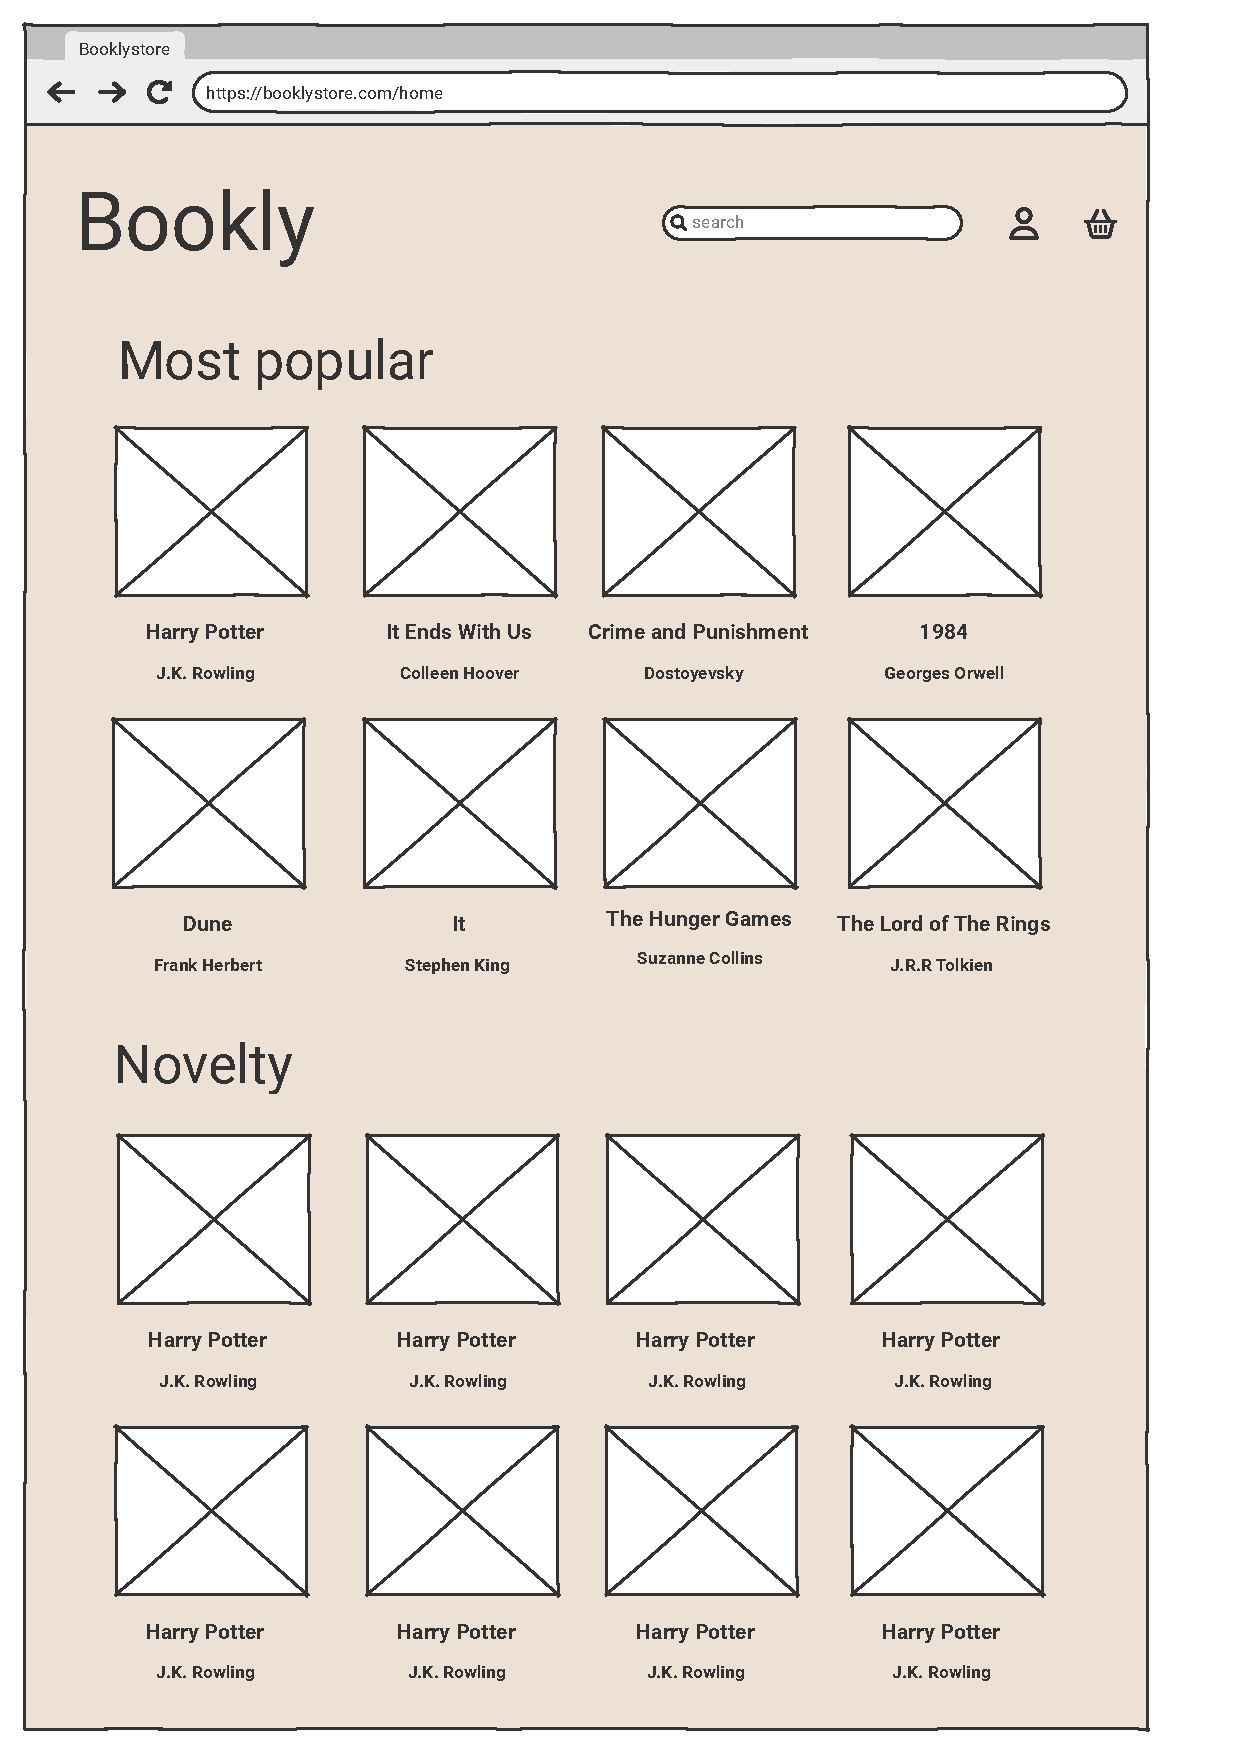
\includegraphics[width=\textwidth]{../photos/homepage.pdf}


\subsection{Sign In/Sign Up Page} \label{sec:signin}
This page allows users to register or log in to their accounts. It includes fields for username, password, an option for password recovery, and a button leading to the Sign-up Page.

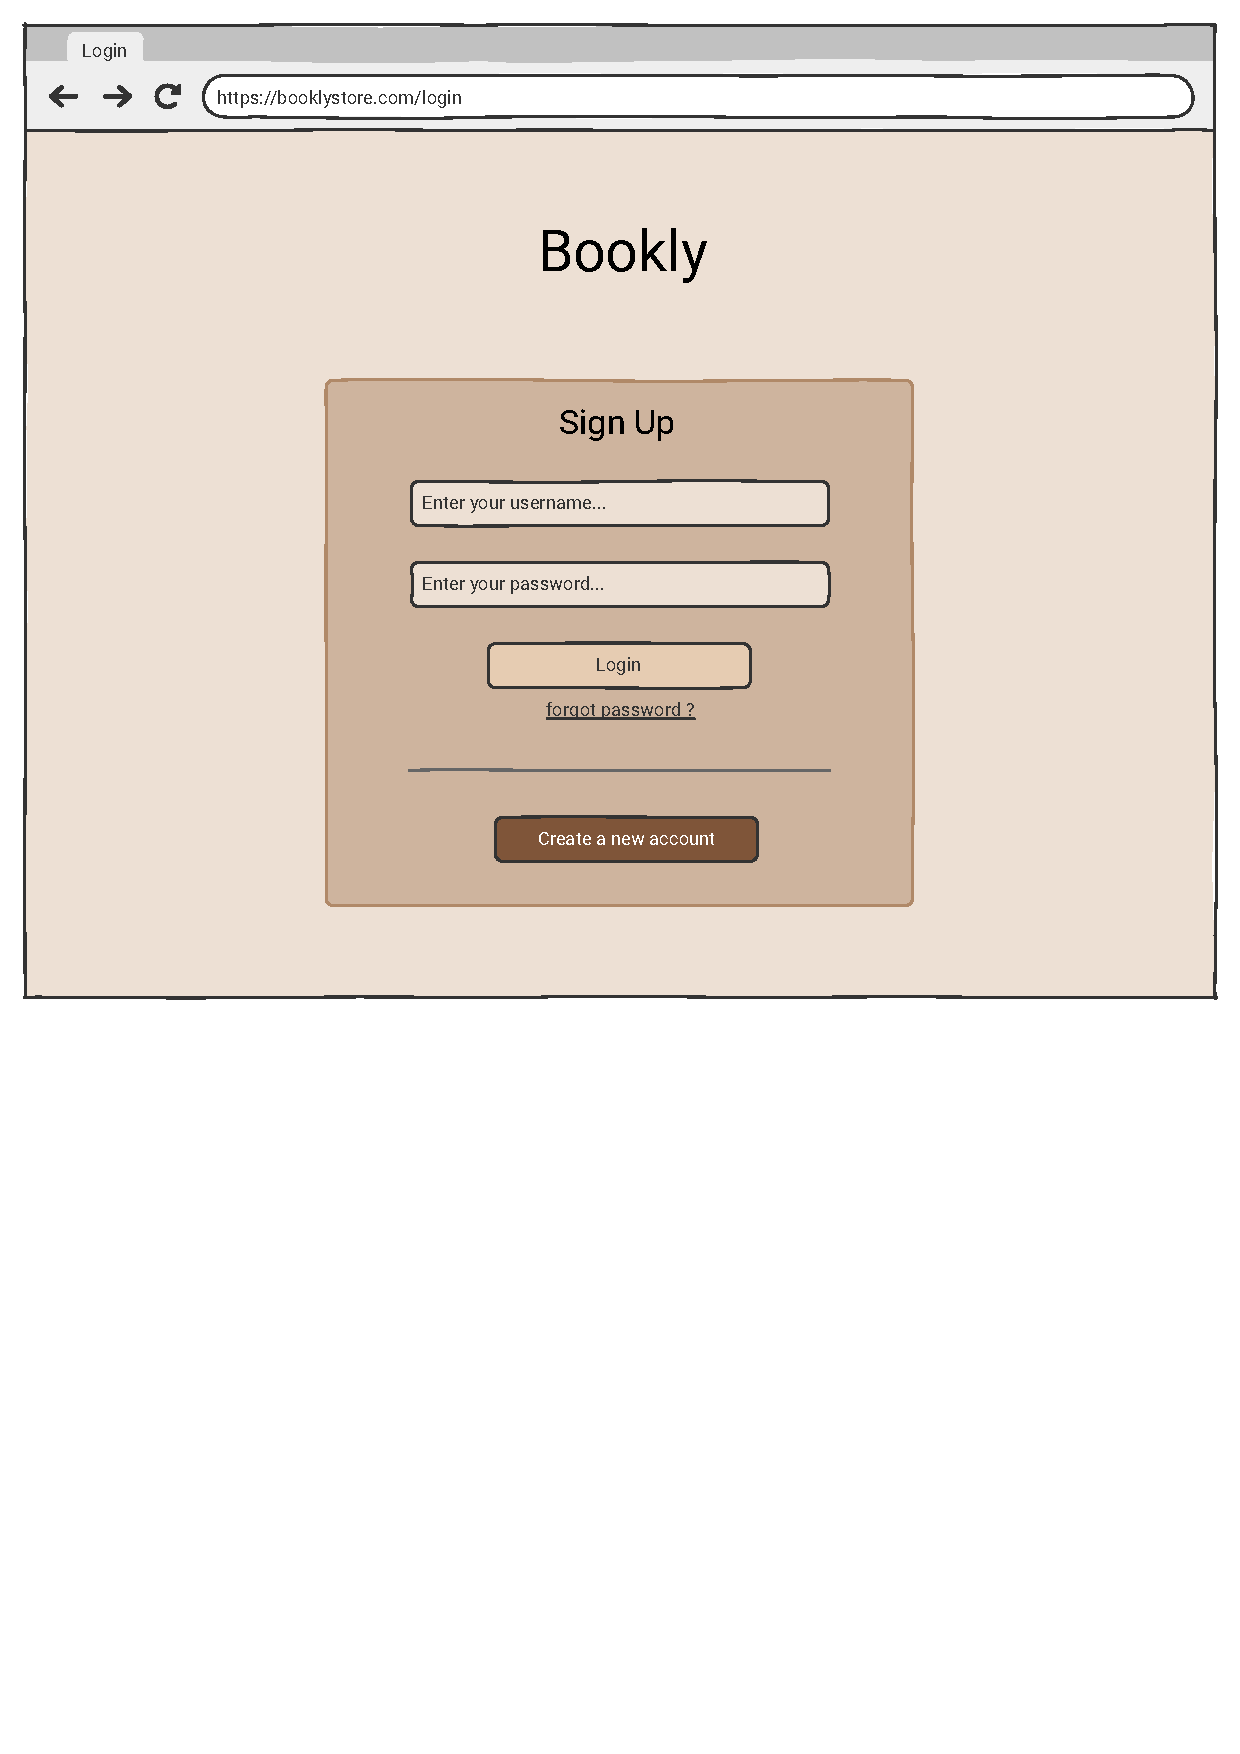
\includegraphics[width=\textwidth]{../photos/signin.pdf}

\subsection{User Profile Page} \label{sec:profile}
Users can also access their profile page, which displays their personal details and order history.

\subsection{Book Page} \label{sec:book}
Each book will have its own dedicated page containing details such as title, author, price, edition, genre, and description. It will also include a review section and a button to add the book to the basket.

\subsection{Basket Page} \label{sec:basket}
This page will show the books added by the user, along with options to update quantities or proceed to checkout.

\subsection{Search Results Page} \label{sec:search}
When a user enters a query in the search bar, they will be redirected to this page, where relevant books will be displayed based on title, author, or genre.